% !TEX TS-program = pdflatex
% !TEX encoding = UTF-8 Unicode

% This is a simple template for a LaTeX document using the "article" class.
% See "book", "report", "letter" for other types of document.

\documentclass[11pt]{article} % use larger type; default would be 10pt

\usepackage[utf8]{inputenc} % set input encoding (not needed with XeLaTeX)

%%% Examples of Article customizations
% These packages are optional, depending whether you want the features they provide.
% See the LaTeX Companion or other references for full information.

%%% PAGE DIMENSIONS
\usepackage{geometry} % to change the page dimensions
\geometry{a4paper} % or letterpaper (US) or a5paper or....
% \geometry{margin=2in} % for example, change the margins to 2 inches all round
% \geometry{landscape} % set up the page for landscape
%   read geometry.pdf for detailed page layout information

\usepackage{graphicx} % support the \includegraphics command and options

% \usepackage[parfill]{parskip} % Activate to begin paragraphs with an empty line rather than an indent

%%% PACKAGES

\usepackage{setspace}
\usepackage{listings}
\usepackage{hyperref}
\usepackage{color}

\definecolor{dkgreen}{rgb}{0,0.6,0}
\definecolor{gray}{rgb}{0.5,0.5,0.5}
\definecolor{mauve}{rgb}{0.58,0,0.82}

\lstset{frame=L,
  language=Python,
  aboveskip=3mm,
  belowskip=3mm,
  showstringspaces=false,
  columns=flexible,
  basicstyle={\small\ttfamily},
  numbers=none,
  numberstyle=\tiny\color{gray},
  keywordstyle=\color{blue},
  commentstyle=\color{dkgreen},
  stringstyle=\color{mauve},
  breaklines=true,
  breakatwhitespace=true,
  tabsize=3
}

\usepackage{booktabs} % for much better looking tables
\usepackage{array} % for better arrays (eg matrices) in maths
\usepackage{paralist} % very flexible & customisable lists (eg. enumerate/itemize, etc.)
\usepackage{verbatim} % adds environment for commenting out blocks of text & for better verbatim
\usepackage{subfig} % make it possible to include more than one captioned figure/table in a single float
% These packages are all incorporated in the memoir class to one degree or another...

%%% HEADERS & FOOTERS
\usepackage{fancyhdr} % This should be set AFTER setting up the page geometry
\pagestyle{fancy} % options: empty , plain , fancy
\renewcommand{\headrulewidth}{0pt} % customise the layout...
\lhead{}\chead{}\rhead{}
\lfoot{}\cfoot{\thepage}\rfoot{}

%%% SECTION TITLE APPEARANCE
\usepackage{sectsty}
\allsectionsfont{\sffamily\mdseries\upshape} % (See the fntguide.pdf for font help)
% (This matches ConTeXt defaults)

%%% ToC (table of contents) APPEARANCE
\usepackage[nottoc,notlof,notlot]{tocbibind} % Put the bibliography in the ToC
\usepackage[titles,subfigure]{tocloft} % Alter the style of the Table of Contents
\renewcommand{\cftsecfont}{\rmfamily\mdseries\upshape}
\renewcommand{\cftsecpagefont}{\rmfamily\mdseries\upshape} % No bold!

%%% END Article customizations

%%% The "real" document content comes below...

\title{Accidental Deaths and Injuries Data Analasys}
\author{
Anja Miletić\\
\texttt{97/2015}
\and
Mateja Marjanović\\
\texttt{172/2015}
}
%\date{} % Activate to display a given date or no date (if empty),
         % otherwise the current date is printed 

\begin{document}
\pagenumbering{gobble}
\maketitle
\newpage

\doublespacing
\tableofcontents
\singlespacing
\newpage

\pagenumbering{arabic}

\section{Uvod}
Podaci su skinuti na linku \url{http://www.gunviolencearchive.org/reports}. Podaci se nalaze u dve datoteke: deaths.csv i injuries.csv i predstavljaju izvestaje o 
slucajnim povredama i smrtnim slucajevima nastalim koriscenjem vatrenog oruzja u Sjedinjenim Americkim Drzavama. 

\section{Analiza i pretprocesiranje podataka}
Obe datoteke sadrze tabele sa istim kolonama. Opisi kolona su dati u tabeli 1.
\newline\newline
\begin{tabular}{|l|l|}
\hline
Incident Date & datum incidenta u obliku Mesec dan, godina \\
\hline
State & savezna americka drzava u kojoj se dogodio incident \\
\hline
City or County & grad ili okrug u kome se dogodio incident \\
\hline
Adress & adresa na kojoj se dogodio incident \\
\hline
\# Killed & broj ubijenih osoba \\
\hline
\# Injured & broj povredjenih osoba \\
\hline
\end{tabular}

\subsection{Analiza podataka}
Pogledajmo detaljnije nase dve datoteke. Koristimo Python kod da izlistamo osnovne informacije o podacima.
\begin{lstlisting}
import pandas

print("**************\n*deaths.csv*\n**************\n")
df_deaths = pandas.read_csv("deaths.csv")
print(df_deaths.head())
print(df_deaths.count())
print(df_deaths.describe())
for col in df_deaths.columns:
    print("count values in column " + col)
    print(df_deaths[col].value_counts(dropna = False))
\end{lstlisting}
rezultat izvrsavanja:
\begin{lstlisting}
**************
*deaths.csv*
**************

     Incident Date   State  City Or County  Address  # Killed  # Injured  Operations
0  August 17, 2018   Louisiana  West Monroe  Philpot Rd   1        0      NaN
1  August 16, 2018   Virginia  Richmond  5600 .. Ct          1      0     NaN
2  August 15, 2018   Kentucky   Louisville    1708 .. St      1      0     NaN
3  August 15, 2018   Ohio       Columbus 1200 .. Rd        1      0     NaN
4  August 14, 2018   Michigan Pontiac   40 .. Salee Ln      1      0    NaN

Incident Date     500
State             500
City Or County    500
Address           468
# Killed          500
# Injured         500
Operations          0

        # Killed   # Injured  Operations
count  500.00000  500.000000         0.0
mean     1.00600    0.038000         NaN
std      0.09992    0.211294         NaN
min      0.00000    0.000000         NaN
25\%      1.00000    0.000000         NaN
50\%      1.00000    0.000000         NaN
75\%      1.00000    0.000000         NaN
max      2.00000    2.000000         NaN

count values in column Incident Date
March 4, 2018         6
July 1, 2017          5
March 12, 2018        5
October 29, 2017      5
November 2, 2017      4
September 30, 2017    4
June 24, 2017         4
May 22, 2018          4
January 1, 2018       4
March 31, 2018        4
February 20, 2018     4
July 4, 2017          4
October 7, 2017       4
June 1, 2017          4
June 8, 2017          4
..
count values in column State
Texas             48
Tennessee         30
Florida           26
Georgia           24
Missouri          23
Ohio              22
Alabama           22
Louisiana         21
Mississippi       21
South Carolina    19
Pennsylvania      17
..
count values in column # Killed
1    495
2      4
0      1
count values in column # Injured
0    483
1     15
2      2
count values in column Operations
NaN    500
\end{lstlisting}
Iz ovih rezultata mozemo primetiti vise stvari. Tabela ima tacno 500 unosa, pri cemu kolone Incident Date, State, City or County, \#Killed i \#Injured nemaju nijednu null vrednost. 
Kolona Operations nema nijednu vazecu vrednost i ona ce biti izbacena iz daljeg razmatranja. Najvise unosa je bilo 4. marta 2018, a najvise incidenata se dogodilo u Teksasu, cak 48.
Kolonu koja predstavlja adrese cemo u nastavku ignorisati. 
\begin{lstlisting}
#remove column Adress and Operations
df = df[['Incident Date','State','City Or County','# Killed','# Injured']]
\end{lstlisting}
Primetimo da u datoteci deaths.csv postoje unosi gde je bilo 0 smrtnih slucajeva. Analogno, u datoteci injuries.csv postoje unosi u kojima nije bilo povredjenih. Ove redove tabele zelimo da izbacimo.
Ovo postizemo uz pomoc sledece dve funckije:
\begin{lstlisting}
import pandas

def no_deaths():
    print('put Null values on zero death rows')
    df_deaths = pandas.read_csv('./deaths.csv')
    for i, row in df_deaths.iterrows():
        number_deaths = row['# Killed']
        if(number_deaths == 0):
            df_deaths.set_value(i, '# Killed', None)

    return df_deaths

def remove_missing_values(df):
    df_deaths_tmp = df[pandas.notnull(df['# Killed'])]
    return df_deaths_tmp
\end{lstlisting}
\subsection{Distribucija frekvencija podataka}
U ovom delu cemo se fokusirati na prvu kolonu tabele, Incident Date. Zelimo da analiziramo frekvenciju incidenata u odnosu na dan u nedelji, mesec i slicno.
Da bi mogli da koristimo unose iz ove kolone moramo da transformisemo datum iz jedne niske u brojcane vrednosti za dan, mesec i godinu koje onda mozemo
da cuvamo u nizovima. Sledeca funkcija konvertuje datum u datetime format:
\begin{lstlisting}
import pandas
from datetime import datetime as dt

def dayofweek(df):
	for i, row in df.iterrows():
		date = row["Incident Date"]
		year_sep = date.split(',')
		date_sep = year_sep[0].split(' ')

		month = months[date_sep[0].strip()]
		day = int(date_sep[1].strip())
		year = int(year_sep[1].strip())

		readable_date = dt.date(year, month, day)

		# 0 - Monday, 6 - Sunday
		y[readable_date.weekday()] += 1
		y_month[month-1] += 1
		if month == 7:
			dayOfJuly[day-1] += 1
\end{lstlisting}
Funckija dayofweek istovremeno kategorise unose prema danu u nedelji i mesecu. Niz dayOfJuly sadrzi sve incidente koji su se dogodili u julu kategorisani po danu.
Koristimo Python biblioteku matplotlib da graficki prikazemo dobijene rezultate.
\begin{lstlisting}
df = pd.read_csv("processed_deaths.csv")

	dayofweek(df)
	print("number of incidents each day of week:")
	print(y)
	plt.bar(x, y, width=0.5, color="blue", tick_label=labels)
	plt.show()

	print("number of incidents per month:")
	print(y_month)
	plt.bar(x_month, y_month, width=0.5, color="red", tick_label=labels_month)
	plt.show()
	
	print("number of incidents per day in july:")
	print(dayOfJuly)
	plt.bar(range(31), dayOfJuly, width=0.5, color="green", tick_label=labels_july)
	plt.show()
\end{lstlisting}
Izlaz u konzoli:
\begin{lstlisting}
number of incidents each day of week:
[ 61.  61.  68.  64.  62. 102.  81.]
number of incidents per month:
[29. 24. 33. 17. 49. 77. 81. 49. 32. 45. 31. 32.]
number of incidents per day in july:
[5. 2. 1. 6. 7. 2. 3. 4. 1. 1. 0. 3. 3. 4. 2. 
0. 1. 1. 2. 3. 1. 4. 2. 4. 0. 3. 3. 2. 4. 4. 3.]
\end{lstlisting}
\begin{figure}[h!]
	\centering
	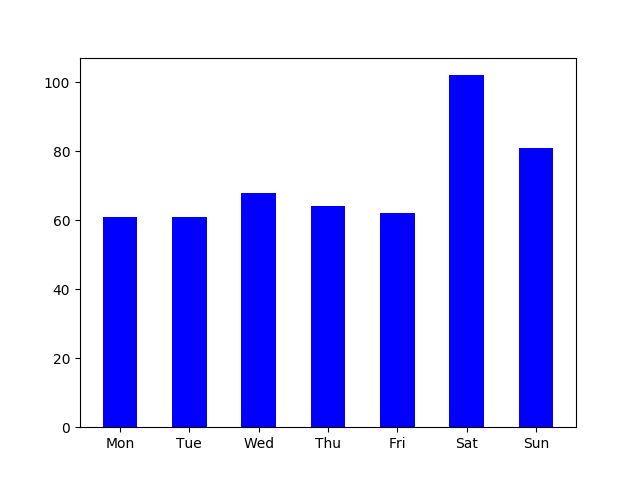
\includegraphics[width=0.8\textwidth]{incidents_per_dayofweek}
	\caption{Distribucija po danu u nedelji}
\end{figure}
\begin{figure}[h!]
	\centering
	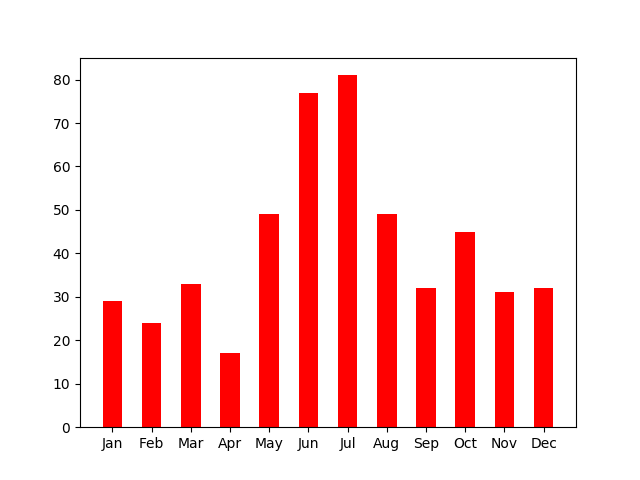
\includegraphics[width=0.8\textwidth]{incidents_permonth}
	\caption{Distribucija po mesecima}
\end{figure}
\begin{figure}[h!]
	\centering
	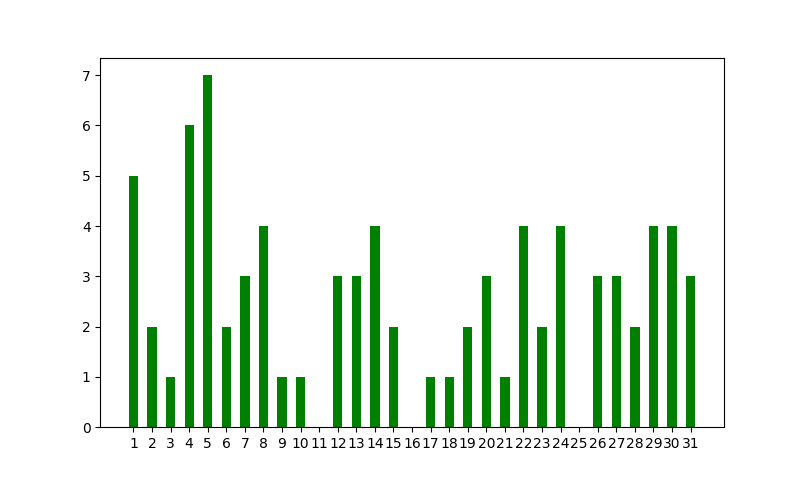
\includegraphics[width=0.8\textwidth]{incidents_july}
	\caption{Distribucija tokom jula}
\end{figure}
Dolazimo do nekoliko zakljucaka; najpre primecujemo ubedljivo najvecu frekvenciju podataka subotom, zatim nedeljom. 
Ovo zapazanje ima smisla jer ljudi vikendom uglavnom ne rade pa stoji da ce se najvise nesreca dogoditi upravo tad.
Zatim, figura 2 pokazuje jun i jul kao mesece u kojima je zabelezeno najvise incidenata, znatno vise nego ostalih 
meseci. Izdvojili smo jul kao mesec od posebnog interesovanja (figura 3). Najvise unosa postoji 4. i 5. jula, iako 
su ovo bili radni dani. Zasto? Upravo tih dana je drzavni praznik u SAD, proslava dana nezavisnosti. Tradicionalno
postoji mnogo veca upotreba oruzja u svrhu proslave ovih dana, a samim tim i veci broj zabelezenih povreda i slucajnih 
smrtnih ishoda. Vredi napomenuti da je 2. novembra, na Dan mrtvih koji obelezavaju pripadnici latino populacije takodje
zabelezen veci broj nesreca od ocekivanog.

	
	
	\newpage
	\section{Klasterovanje}
	Proces klasterovanja izvrsen je na podacima koji su pre samog izvrsavanja pripremljeni (pretprocesiranje i namestanje podataka). 
	Podaci koji su prosledjeni imaju dva atributa, to su 'State' i 'Number of Incidents', 'State' predstavlja drzavu, a 'Number of Incidents' predstavlja 
	ukupan broj incidenata (slucajnih povreda i slucajnih ubistava) u toj drzavi.
	
	\subsection{Pripremanje podataka za klasterovanje}
	Da bismo izvrsili klasterovanje koje ima smisla, gde moze da se vidi koji podaci su slicniji, a koji razlicitiji, moramo da prvo te podatke izmenimo na 
	neki nacin i namestimo ih da budu takvi da nam odgovaraju. U narednom kodu napisanom u Python-u smo izmenili podatke iz 
	processed\_deaths.csv i processed\_injuries.csv i napravili novi fajl summedIncidentsPerState.csv.
	\newline
	
	\begin{lstlisting}
def changeDateFormat(df):
	for i, row in df.iterrows():
		month = row["Incident Date"].strip().split(' ')[0].split(',')[0]
		df.set_value(i, "Incident Date", month)
	
	df = df.drop(columns = ["Unnamed: 0", "Incident Date", "City Or County"])
	
	allIncidents = {}
	allStates = []
	for i, row in df.iterrows():
		state = row["State"].strip()
		if state not in allStates:
			allStates.append(state)
			allIncidents[state] = int(row["# Injured"]) + int(row["# Killed"])
		else:
			allIncidents[state] += int(row["# Injured"]) + int(row["# Killed"])
		df = df.drop([i])
	
	df = df.drop(columns = ["# Killed", "# Injured"])
	for k, v in allIncidents.iteritems():
		state = k
		numberOfDeaths = v
		df = df.append({"State" : state, "# Incidents" : int(numberOfDeaths)}, ignore_index = True)
	
	return df
	
    \end{lstlisting}
	
	\subsection{Prosledjivanje generisanih podataka i klasterovanje}
	Sad kad smo generisali podatke koristimo ih u Knime-u.
	Prvo citamo podatke sa CSV Reader-om, zatim ih saljemo na normalizaciju, tj. da se vrednosti iz kolone sa brojem ubistava skaliraju na interval [0, 1].
	Posle toga racunamo Euklidska rastojanja podataka, pa ta rastojanja i izlaz iz cvora koji je normalizovao podatke saljemo DBSCAN cvoru koji 
	dodaje jos jednu kolonu i svakoj instanci dodeljuje neku vrednost u zavisnosti od toga gde se nalazi.
	Ostalo je samo jos da se iscrtaju podaci, da bismo to uradili koristimo Color Manager i Scatter Plot.
	\newline
	
	\begin{figure}[h!]
	\centering
		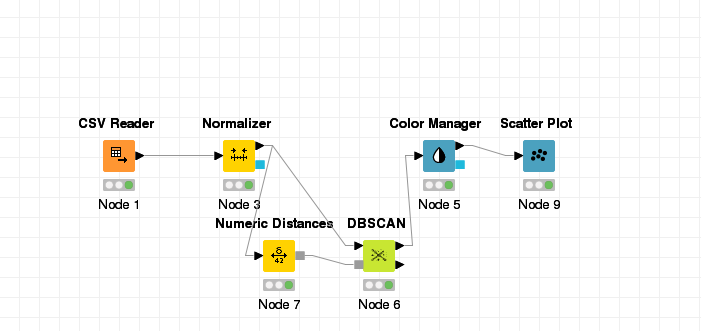
\includegraphics[width=0.8\textwidth]{klasterovanjeKnime}
		\caption{Izgled klasterovanja podataka u Knime-u}
	\end{figure}
	
	
	\newpage
	\subsection{Izgled klasterovanih podataka i analiza}
	Sada imamo podatke koji su podeljeni, svaki pripada nekom klasteru (neki pripadaju klasteru Noise) i svakom klasteru je dodeljena druga boja. Moze se 
	primetiti da je drzava u kojima ima vise ubistava mnogo manje nego drzava u kojima ima imanje. Npr. u Teksasu ima toliko vise nego bilo gde drugde da se 
	Teksas dozivljava kao sum.
	
	\begin{figure}[h!]
	\centering
		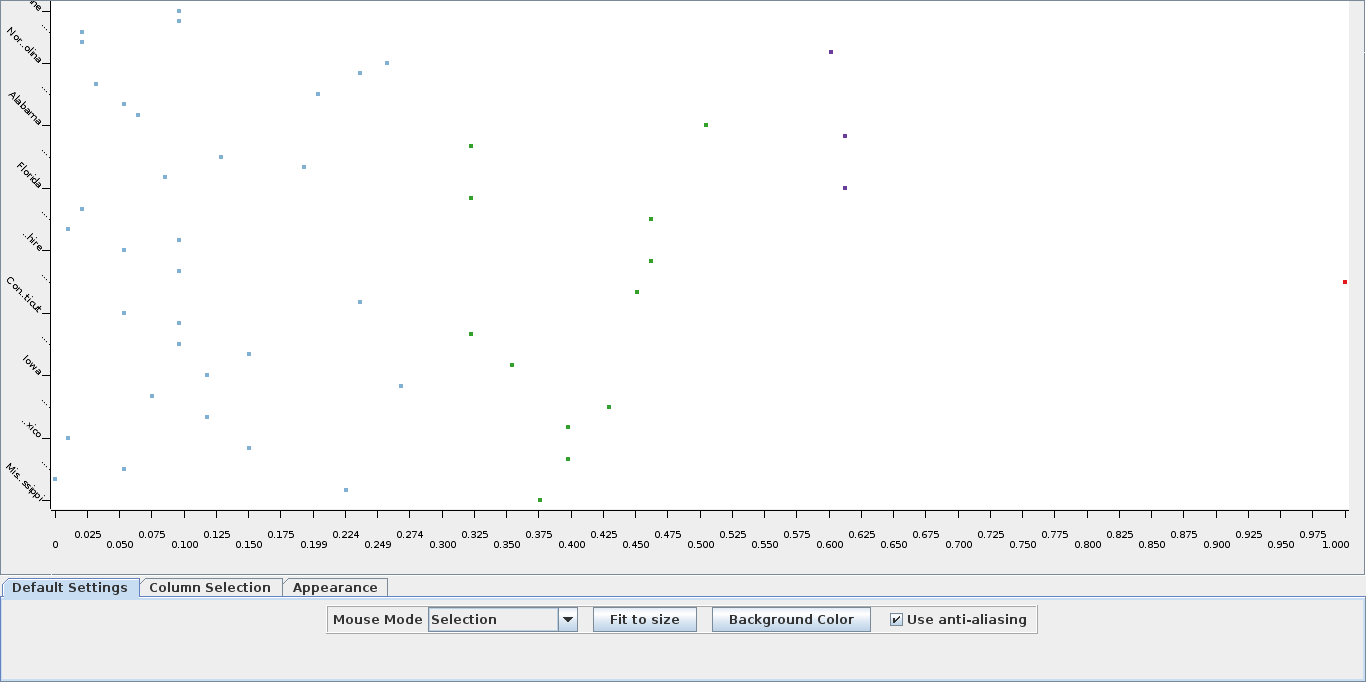
\includegraphics[width=0.8\textwidth]{klasterovanje1}
		\caption{Klasterovani podaci koji prikazuju zavisnost drzave i broja ubistava u toj drzavi}
	\end{figure}
	
	\newpage
	\section{Klasifikacija}
	Proces klasifikacije ili nadgledanog ucenja slicno kao i klasterovanje izvrsavamo na podacima koje smo generisali u drugom programu, zatim smo u 
	Knime-u te podatke iskoristili i izvrsili klasifikaciju. 
	Uradjene su dve klasifikacije. 
	Jedna je predvidjanje da li ce u odredjenom danu u nedelji u odredjenom mesecu biti malo, srednje ili puno incidenata. 
	Malo incidenata znaci da se u tom mesecu, u tom danu u nedelji (npr. svakom ponedeljku) ukupno desilo manje od 8, srednje znaci da je taj broj izmedju 8 i 15, 
	a puno vise od 15. Sa ovim brojevima ima slican broj parova (dan u nedelji, mesec) (blizu 33\% svako). To nije slucajnost, s obzirom na to da je 
	uzoracka sredina broja ubistava 12.8.
	U drugoj klasifikaciji izvrsava se predvidjanje da li ce biti puno (vise od 1) ili malo (manje jednako 1) incidenata u nekoj drzavi u nekom gradu.
	
	\subsection{Klasifikacija: Dan u nedelji, mesec, broj incidenata}
	Kao i ranije prvo podatke zelimo da transformisemo i dobijemo zeljeni oblik. U ovom slucaju zeljeni oblik bi bio da imamo kolonu mesec, dan u nedelji i 
	ukupan broj incidenata u toj kombinaciji (meseca i dana u nedelji). Sledeci kod ce generisati novi fajl u kome ce se nalaziti podaci.

	\begin{lstlisting}
def changeDateFormat(df):
	df = df.drop(columns = ["Unnamed: 0", "Incident Date"])
	
	incidents = {}
	for i, row in df.iterrows():
		state = row["State"].strip()
		city = row["City Or County"].strip()
		if state + ":" + city not in incidents:
			incidents[state + ":" + city] = int(row["# Injured"]) + int(row["# Killed"])
		else:
			incidents[state + ":" + city] += int(row["# Injured"]) + int(row["# Killed"])
		df = df.drop([i])
	
	df = df.drop(columns = ["# Killed", "# Injured"])
	for k, v in incidents.iteritems():
		key = k.split(':')
		city = key[1]
		state = key[0]
		numberOfDeaths = v
		df = df.append({"State" : state, "City Or County" : city, "# Incidents" : int(numberOfDeaths)}, ignore_index = True)
	
	return df
	\end{lstlisting}
	
	\subsubsection{Klasifikacija u Knime-u}
	
	\begin{figure}[h!]
        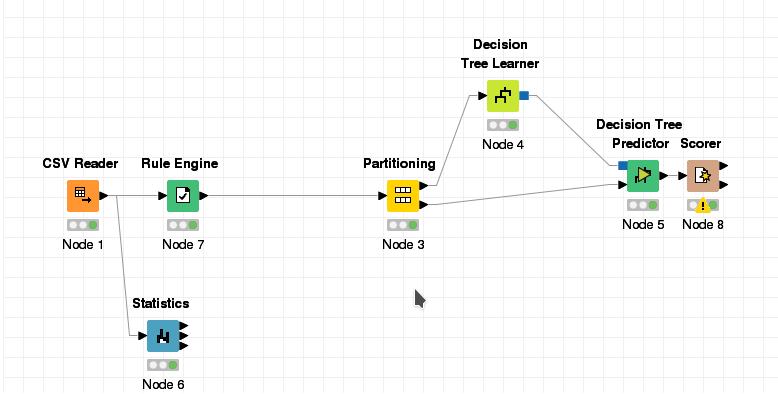
\includegraphics[width=0.8\textwidth]{klasifikacijaDanMesecKnime}
        \caption{Izlged klasifikacije u Knime-u}
	\end{figure}
	
	\begin{figure}[h!]
        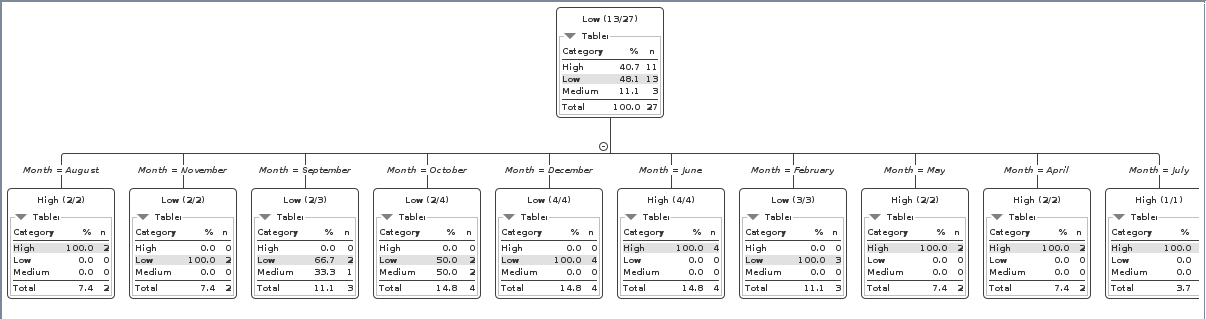
\includegraphics[width=0.8\textwidth]{klasifikacijaDanMesec}
        \caption{Drvo odlucivanja u kome se na osnovu dana u nedelji i meseca predvidja da li ce biti malo, srednje ili puno incidenata}
	\end{figure}
	
	\begin{figure}[h!]
        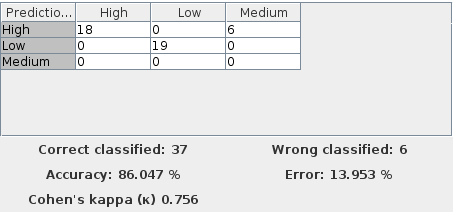
\includegraphics[width=0.8\textwidth]{matricaKonfuzije}
        \caption{Matrica konfuzije}
	\end{figure}
	
\end{document}






























